\section{Test og konklusion}

Sideløbende med udviklingen af systemet er al funktionalitet testet. Der er ikke sat nogle automatiske test op, men da AVR Dragon er brugt som debugværktøj har det alligevel været hurtigere end ellers at teste system. Dette skyldes at det ikke har været nødvendigt at gå den ''lange vej'' gennem Atmel Studio's \textit{Device Programmer}.

\subsection{Test}

Billedet i figur~\ref{fig:testsetup} viser opstillingen for test. Her er der simpelthen sendt de forskellige kommandoer til GSM modulet pr. SMS og efterfølgende er det ved manuel aflæsning konstateret hvorvidt det rigtige response er kommet.

\begin{figure}[h]
	\centering
	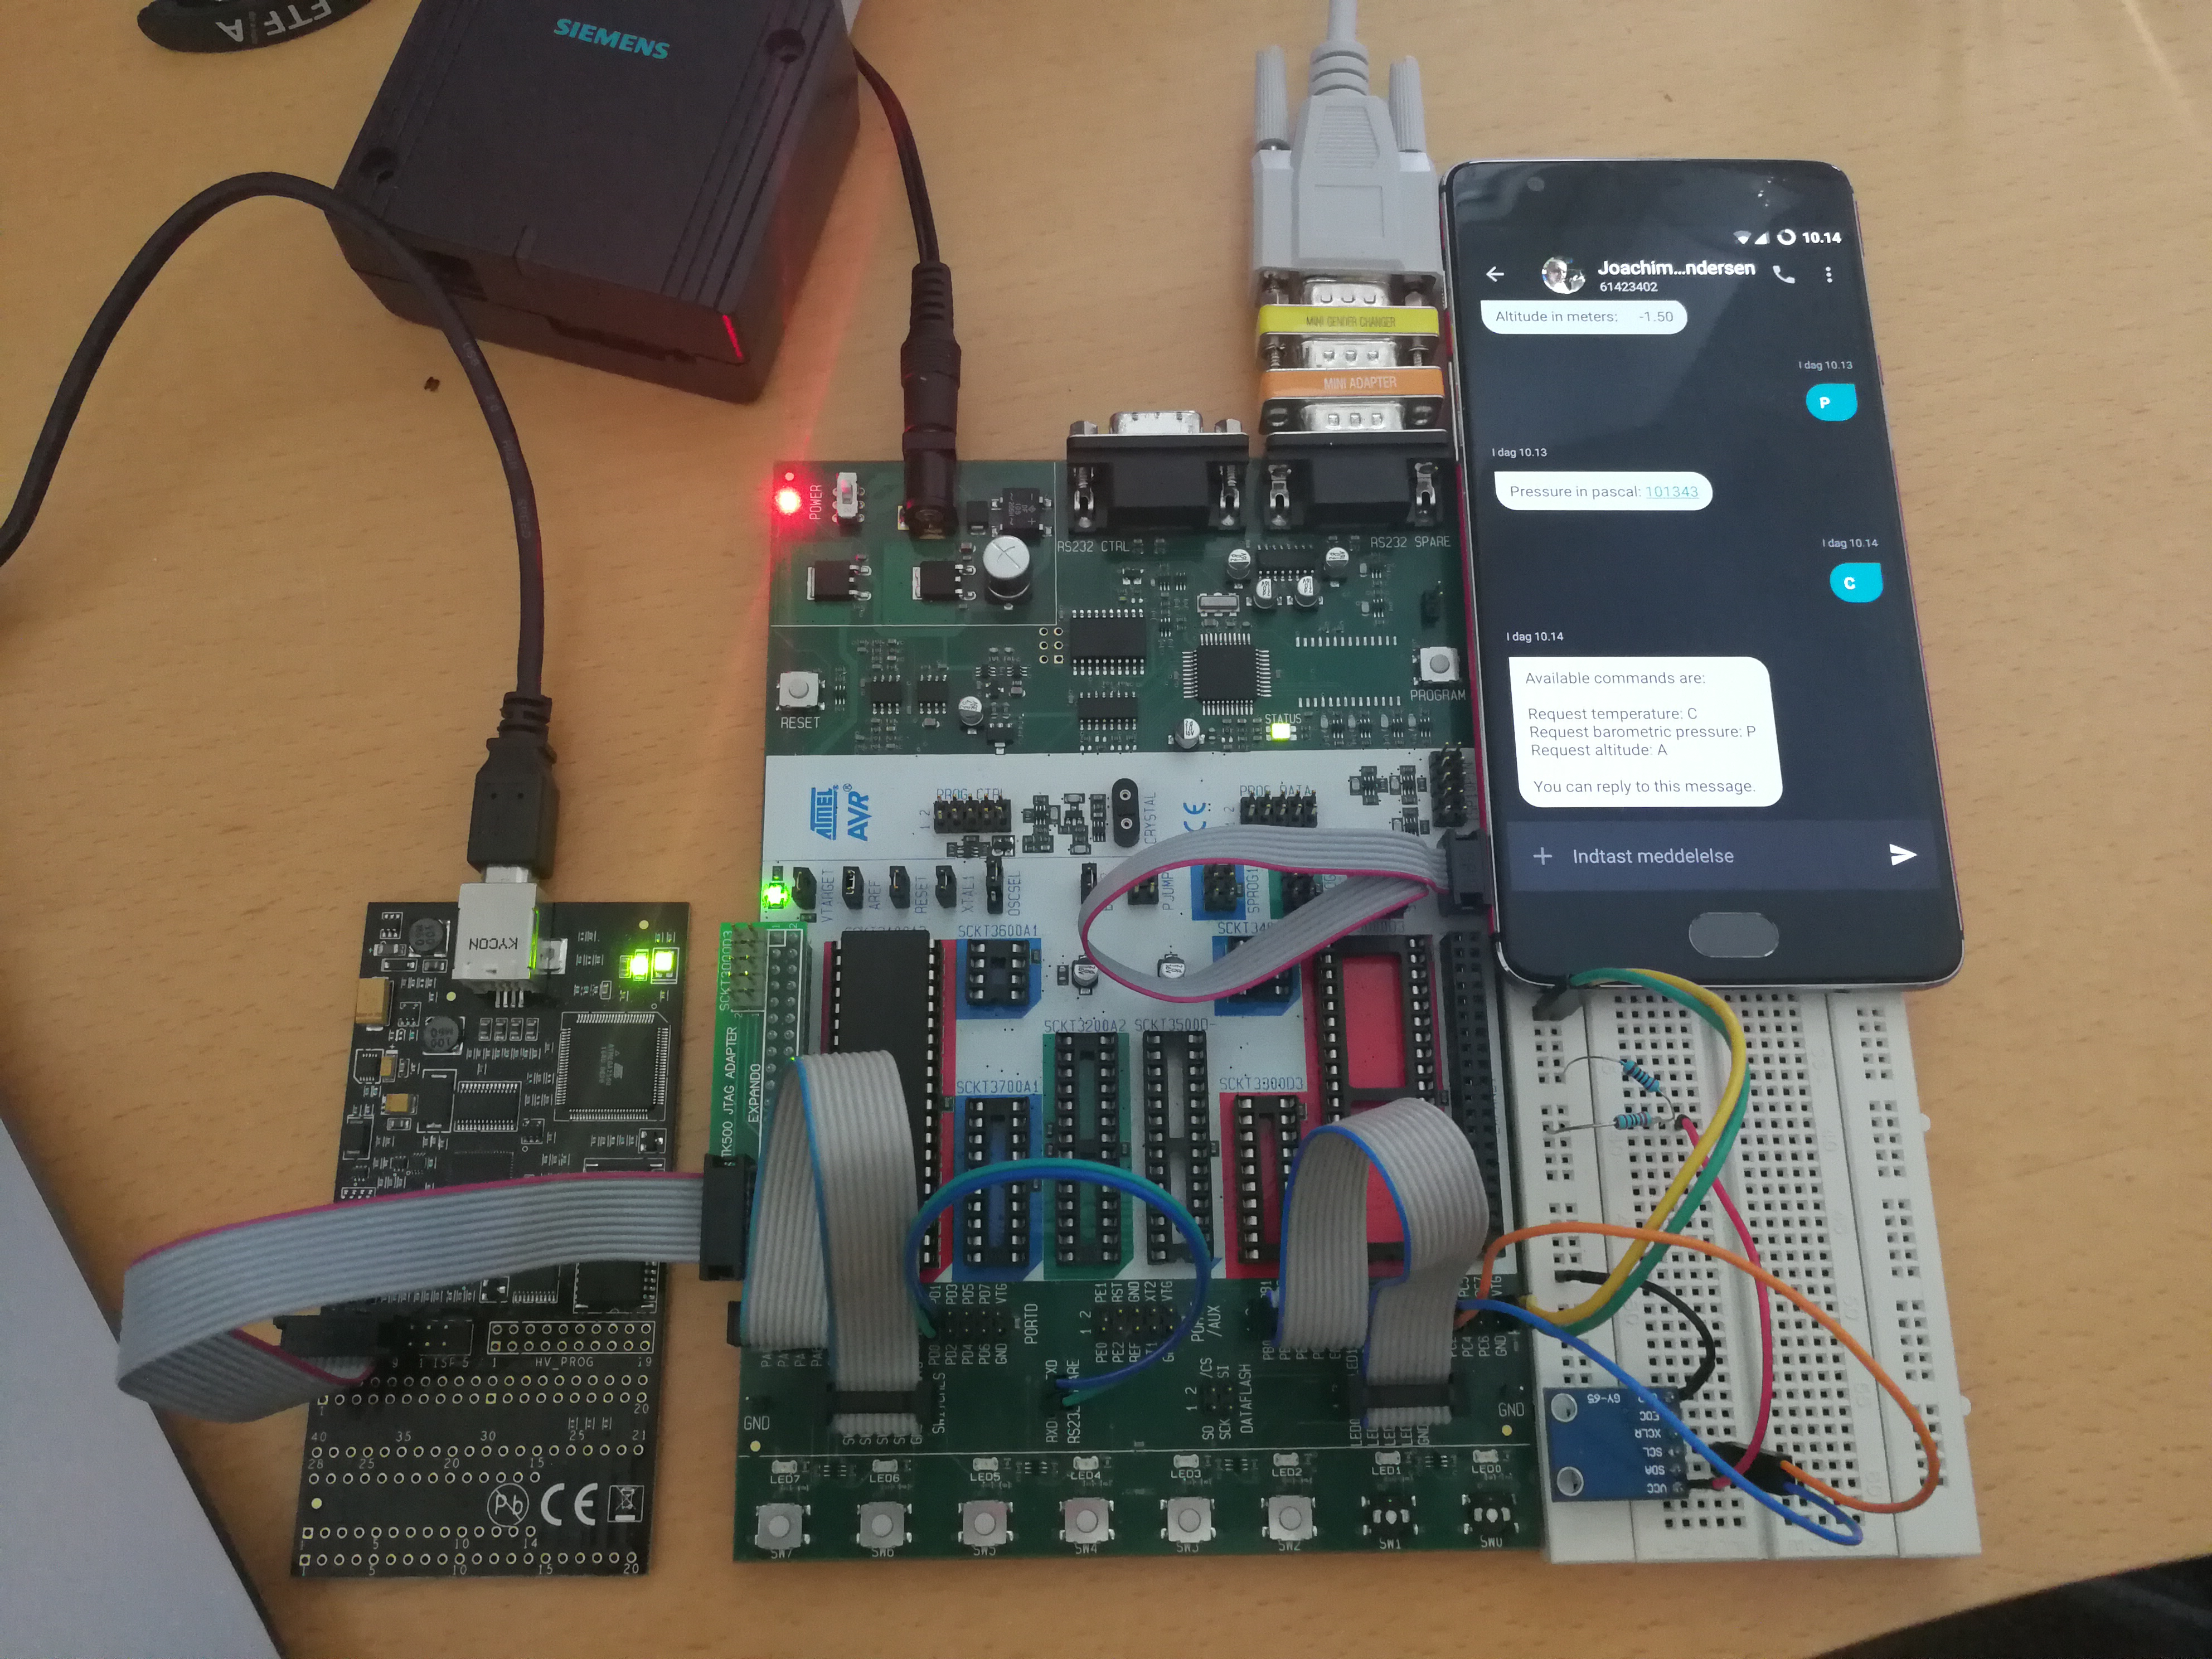
\includegraphics[width=\linewidth]{figs/test_setup}
	\caption{Billede af testopsætning.}
	\label{fig:testsetup}
\end{figure}

\subsection{Demo}
Da demo-guderne næppe tillader at en ''live''-demo går godt, er herunder et link til en YouTube video, som demonstrerer systemet.

\vskip 0.5cm
	\begin{center}
		\url{https://www.youtube.com/watch?v=xx1EggCptEE}
	\end{center}
\vskip 0.5cm

\subsection{Konklusion}

I løbet af dette projekt er det lykkedes at udvikle et system som ved modtagelse af en SMS kan indhente en sensormåling fra ekstern enhed og svare på den oprindelige besked med den ønskede måling. 

Den største udfordring har været at få MC35 GSM modem'ets timings til at stemme med kravene fra fabrikken. Men da disse udfordringer var løst kunne de resterende opgaver relativt hurtigt løses.

Alt i alt er projektet gået godt og den valgte problemstilling er blevet løst efter hensigt. 